\chapter{Introdução}
%\markboth{\thechapter ~~~ Introdução}{}
%\label{intro}

Um sistema pode ser visto como um processo com sinais de entrada que são 
transformados ou induzidos a responder de alguma forma, resultando em outros 
sinais de saída \cite{Oppenhein}. O intuito do controlador é manipular o sistema com a 
finalidade de obter um sinal de saída que seja desejado. A implementação do 
controlador é fundamental para tornar possível processos em diferentes áreas como 
sistemas eletrônicos de potência \cite{Rothstein}, acionamentos elétricos 
\cite{Bouscayrol}, engenharia de tráfego \cite{Bullock} e robótica móvel 
\cite{Kamali}. Para isso, os sistemas são modelados matematicamente através de 
equações diferenciais lineares, e o controlador é projetado a partir do modelo 
matemático.

No controle em malha aberta, a saída não exerce nenhuma ação sobre o sinal de 
controle. Desta forma, aplica-se um sinal na entrada de uma planta ou de um 
processo para que a variável controlada atinja um valor desejado, mas este 
valor obtido na saída não é utilizado para modificar a entrada. O problema 
deste tipo de controle é que o sistema pode adquirir novas características 
, por exemplo, ao ocorrerem perturbações. Caso isso ocorra, a saída não 
terá o valor desejado anteriormente.

Ao fechar a malha, o sinal de saída passa a interferir diretamente na ação de 
controle. Assim, o sistema ganha o conceito de realimentação e erro, 
e o controlador tende a reduzir o erro (deferença entre os valores de referência 
e realimentação) e a manter a saída no valor desejado. ``Controlar a saída de 
uma planta ou de um processo por realimentação significa aplicar na sua entrada, 
após conveniente amplificação, o sinal resultante da 
diferença entre o valor desejado e o valor medido da saída \cite[p.~3]{Castrucci}.''

A simulação \emph{Hardware in the Loop} (HIL) é uma técnica bem estabelecida 
usada em projeto e avaliação de sistemas de controle \cite{Bacic}. Esta técnica de 
controle consiste em projetar o controlador para uma determinada planta 
substituindo o bloco de controle $C(s)$ na Figura \ref{fig:diagBloco} por um 
microcontrolador físico e validando o desempenho do sistema em malha fechada com 
esse controlador, como ilustrado na Figura \ref{fig:diagBlocoHIL}.

\begin{figure}[ht]
  \centering
  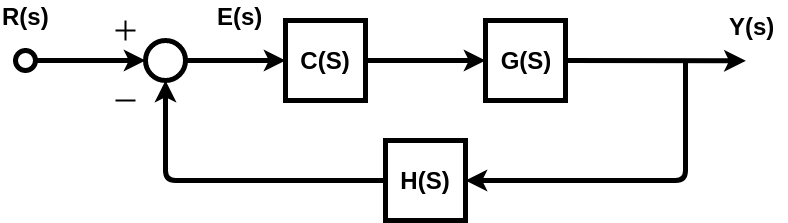
\includegraphics[width = 0.6\columnwidth]{Imagens/blocosMF.png}
  \caption{Diagrama de blocos do sistema em malha fechada}
  \label{fig:diagBloco} 
\end{figure}

\begin{figure}[ht]
  \centering
  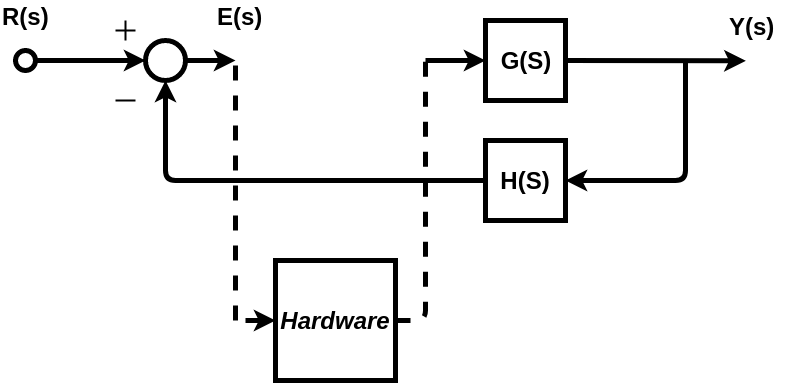
\includegraphics[width = 0.7\columnwidth]{Imagens/blocoHard.png}
  \caption{Diagrama de blocos do sistema em malha fechada - \emph{Hardware in the Loop}}
  \label{fig:diagBlocoHIL} 
\end{figure}

% O que este PFC pretende alcançar e como? Metodologia a ser seguida.

O controle em malha fechada utiliza a informação de como a variável controlada evolui 
para determinar o sinal de controle aplicado ao processo. Determinado o modelo da 
planta a ser controlada, o controlador é sintonizado de forma a atender especificações 
de projeto fornecidas. Geralmente, 
uma vez sintonizado o controlador e validado o desempenho em malha fechada da 
planta realimentada, passa-se a implementação prática do controle sem que haja 
uma prévia validação do comportamento do controlador quando implementado em 
dispositivo físico. 

O controle da planta possui três etapas distintas de execução. A primeira trata-se 
do projeto do controlador simulado em conjunto com o modelo da planta; a segunda 
é a implementação em dispositivo físico do controlador e validação com 
o modelo da planta; e a terceira trata-se da validação da estratégia de controle 
na planta física.

\section{Motivação e Justificativa}
\markright{\thesection ~~~ Motivação e Justificativa}
%\label{motiva}

Nos dias de hoje, as simulações \emph{Hardware in the Loop} (HIL) são utilizadas
cada vez mais para desenvolverem novos componentes e atuadores em vários campos
diferentes \cite{Bouscayrol}. A ação de controle agora não depende 
apenas da computação numérica, mas também da forma como o modelo interage com um 
equipamento de controle externo. Além disso, o conceito de sistemas embarcados 
exige cada vez mais o uso de ferramentas independentes encarregadas de executar 
uma função específica.

Sabe-se que os seres humanos têm limitações para frequentar determinados ambientes, 
principalmente os ambientes industriais, onde estão submetidos a alta insalubridade 
\cite{Lacaz}. Consequentemente, nos últimos anos, tem sido cada vez mais frequente 
em indústrias, o uso de tecnologias que visam automatizar seus processos de 
fabricação. Estas soluções visam a melhoria na qualidade do trabalho, e, 
consequentemente, um aumento de produtividade. Os manipuladores robóticos são 
exemplos de soluções deste tipo, sejam eles controlados remotamente, ou totalmente independentes 
da ação humana. A maior parte das aplicações de manipuladores está voltada para a indústria, 
principalmente as que utilizam linhas de produção (como montadoras e fabricantes de autopeças)
\cite{Spong}.

\section{Objetivos do Projeto}
\markright{\thesection ~~~ Objetivos do Projeto}
%label{objetivos}

O objetivo principal do presente projeto é sintonizar e validar estratégias de 
controle para o sistema dinâmico de um manipulador robótico utilizando a técnica 
\emph{Hardware in the Loop} (HIL). Além disso, será construída uma plataforma de 
validação de controladores através do \emph{Hardware in the Loop} (HIL).

\section{Local de Realização}
\markright{\thesection ~~~ Local de Realização}
%\label{empresa}

Departamento de Engenharia Eletrônica da UFMG (DELT/UFMG). O departamento 
situa-se dentro do campus Pampulha da UFMG na Escola de Engenharia. O campus 
fica na Av. Presidente Antônio Carlos 6627 - Pampulha, Belo Horizonte - MG, 
31270-901.

O departamento foi criado em 1969 e tem contribuído para a formação dos 
engenheiros eletricistas e engenheiros de controle e automação da UFMG. O DELT é 
referência no cenário nacional, e, é também, o Departamento da UFMG com maior 
participação no curso de graduação em Engenharia de Controle e Automação.

\section{Estrutura da Monografia}
\markright{\thesection ~~~ Estrutura da Monografia}
%\label{organizacao}

A monografia está dividida em cinco capítulos. Este capítulo apresentou uma introdução 
ao projeto e o local onde o trabalho foi realizado. O Capítulo 2 descreve 
os princípios básicos de um manipulador robótico e a técnica \emph{Hardware in the 
Loop} (HIL). Ele também abrange todos os conceitos necessários para um melhor 
entendimento do trabalho. O Capítulo 3 aborda a metodologia de desenvolvimento do trabalho. 
Nesse capítulo são feitas a modelagem da planta de estudo e validação do modelo, a 
concepção do ambiente de simulação, as especificações das estratégias de controle no 
microcontrolador e, por fim, as validações das estratégias por meio de simulações. 
Os resultados experimentais são apresentados no Capítulo 4. Primeiramente, a 
metodologia HIL é validada, para diferentes estratégias de controle, no ambiente 
de simulação concebido no Capítulo 3 e, posteriormente, os controladores 
implementados são aplicados à planta física em estudo. 
Finalmente, no capítulo 5, tem-se a conclusão da  monografia com algumas sugestões 
para trabalhos futuros e dificuldades encontradas na realização do projeto.


\clearpage